\chapter{Réalisation et Interfaces}

\section{Introduction}
Ce chapitre détaille la phase d'implémentation technique de ManageraHub. Il décrit l'environnement de développement matériel et logiciel, détaille l'architecture MVT de Django appliquée aux différents modules, justifie les optimisations de requêtes implémentées, présente les écrans finaux de l'application via des conteneurs de captures d'écran, et analyse les difficultés rencontrées lors de la phase d'intégration responsive.

\section{Environnement de travail}
\subsection{Environnement matériel}
Le développement de la plateforme a été réalisé sur une machine portable équipée d'un processeur Intel Core i7 cadencé à 2.8 GHz, de 16 Go de mémoire vive (RAM) et d'un stockage SSD de 512 Go. Cette configuration a permis de faire tourner le serveur de développement local et la base de données relationnelle de manière fluide.

\subsection{Environnement logiciel}
\begin{itemize}
    \item \textbf{Système d'exploitation :} Windows 11 Professionnel.
    \item \textbf{Langage et Framework :} Python (version 3.9) et Django (version 4.2 LTS).
    \item \textbf{IDE / Éditeurs :} Visual Studio Code pour l'écriture et le débogage du code Python\allowbreak/Django et des fichiers statiques.
    \item \textbf{Gestion des versions :} Git pour le contrôle de version, hébergé sur GitHub.
    \item \textbf{Base de données :} MySQL / MariaDB (utilisant la bibliothèque \texttt{PyMySQL}) pour le développement local et la production.
\end{itemize}

\section{Architecture technique du code source}
Le code de ManageraHub est structuré au sein d'une seule application Django principale nommée \texttt{app1} (sous le projet global \texttt{monprojet}). Cette approche centralisée simplifie grandement les imports de modèles et l'architecture globale.

\subsection{Modèles (app1/models.py)}
Voici un exemple d'extrait du fichier de définition de nos modèles de profils CandidateProfile et CompanyProfile, liés au modèle utilisateur par défaut de Django (\texttt{User}) :

\begin{lstlisting}[language=Python, caption=Définition des modèles de profils CandidateProfile et CompanyProfile]
from django.db import models
from django.conf import settings

def candidate_profile_file_path(instance, filename):
    user_id = getattr(instance, "user_id", None)
    if user_id is None and hasattr(instance, "profile_id"):
        user_id = instance.profile.user_id
    return f"candidate_profiles/user_{user_id}/{filename}"

def company_profile_file_path(instance, filename):
    return f"company_profiles/user_{instance.user_id}/{filename}"

class CandidateProfile(models.Model):
    user = models.OneToOneField(
        settings.AUTH_USER_MODEL,
        on_delete=models.CASCADE,
        related_name="candidate_profile",
    )
    phone_number = models.CharField(max_length=40, blank=True)
    address = models.CharField(max_length=255, blank=True)
    city = models.CharField(max_length=120, blank=True)
    country = models.CharField(max_length=120, blank=True)
    education_level = models.CharField(max_length=120, blank=True)
    skills = models.TextField(blank=True)
    experience_summary = models.TextField(blank=True)
    headline = models.CharField(max_length=180, blank=True)
    bio = models.TextField(blank=True)
    profile_picture = models.FileField(upload_to=candidate_profile_file_path, blank=True)
    cv_file = models.FileField(upload_to=candidate_profile_file_path, blank=True)
    cover_letter_file = models.FileField(upload_to=candidate_profile_file_path, blank=True)
    is_public = models.BooleanField(default=True)
    created_at = models.DateTimeField(auto_now_add=True)
    updated_at = models.DateTimeField(auto_now=True)

class CompanyProfile(models.Model):
    user = models.OneToOneField(
        settings.AUTH_USER_MODEL,
        on_delete=models.CASCADE,
        related_name="company_profile",
    )
    company_name = models.CharField(max_length=180, blank=True)
    industry = models.CharField(max_length=120, blank=True)
    company_size = models.CharField(max_length=60, blank=True)
    phone_number = models.CharField(max_length=40, blank=True)
    city = models.CharField(max_length=120, blank=True)
    country = models.CharField(max_length=120, blank=True)
    website = models.URLField(max_length=300, blank=True)
    description = models.TextField(blank=True)
    logo = models.ImageField(upload_to=company_profile_file_path, blank=True)
    background_image = models.ImageField(upload_to=company_profile_file_path, blank=True)
    is_approved = models.BooleanField(default=False)
    ice = models.CharField(max_length=15, blank=True, null=True)
    rc_number = models.CharField(max_length=50, blank=True, null=True)
    legal_document = models.FileField(upload_to=company_profile_file_path, blank=True, null=True)
    created_at = models.DateTimeField(auto_now_add=True)
    updated_at = models.DateTimeField(auto_now=True)
\end{lstlisting}

\subsection{Logique métier (views.py) et optimisation des requêtes BDD}
Afin d'éviter le problème classique des requêtes N+1 (N+1 Query Problem), nous avons optimisé le chargement des publications dans le fil d'actualités social. En utilisant \texttt{select\_}\allowbreak\texttt{related} pour précharger l'auteur du post et l'entreprise taguée, et \texttt{prefetch\_}\allowbreak\texttt{related} pour les commentaires, leurs auteurs et les mentions d'utilisateurs, nous réduisons le nombre de requêtes SQL de plus de 80\% sur les pages de flux social.

\begin{lstlisting}[language=Python, caption=Optimisation des requêtes du Feed social dans views.py]
from django.shortcuts import render
from .models import Post

def candidate_feed_view(request):
    # Optimisation par prechargement select_related et prefetch_related
    posts = Post.objects.select_related("author", "tagged_company").prefetch_related(
        "likes", "comments", "comments__author", "tagged_users", "tagged_users__candidate_profile"
    ).all()
    
    return render(request, 'candidate/feed.html', {'posts': posts})
\end{lstlisting}

\section{Présentation des interfaces de l'application}
Cette section présente la charte graphique implémentée ainsi que les maquettes fonctionnelles et captures d'écran des différents modules de l'application. La charte graphique utilise des nuances de **Dark Plum** (\texttt{\#4F0C28}) comme couleur principale et de **Periwinkle** (\texttt{\#C5D2F8}) comme couleur secondaire pour les accents.

\subsection{1. Page d'accueil et d'authentification}
La landing page présente les services de la plateforme aux visiteurs et propose deux boutons d'appel à l'action distincts pour s'inscrire en tant que candidat ou entreprise.

\begin{figure}[H]
    \centering
    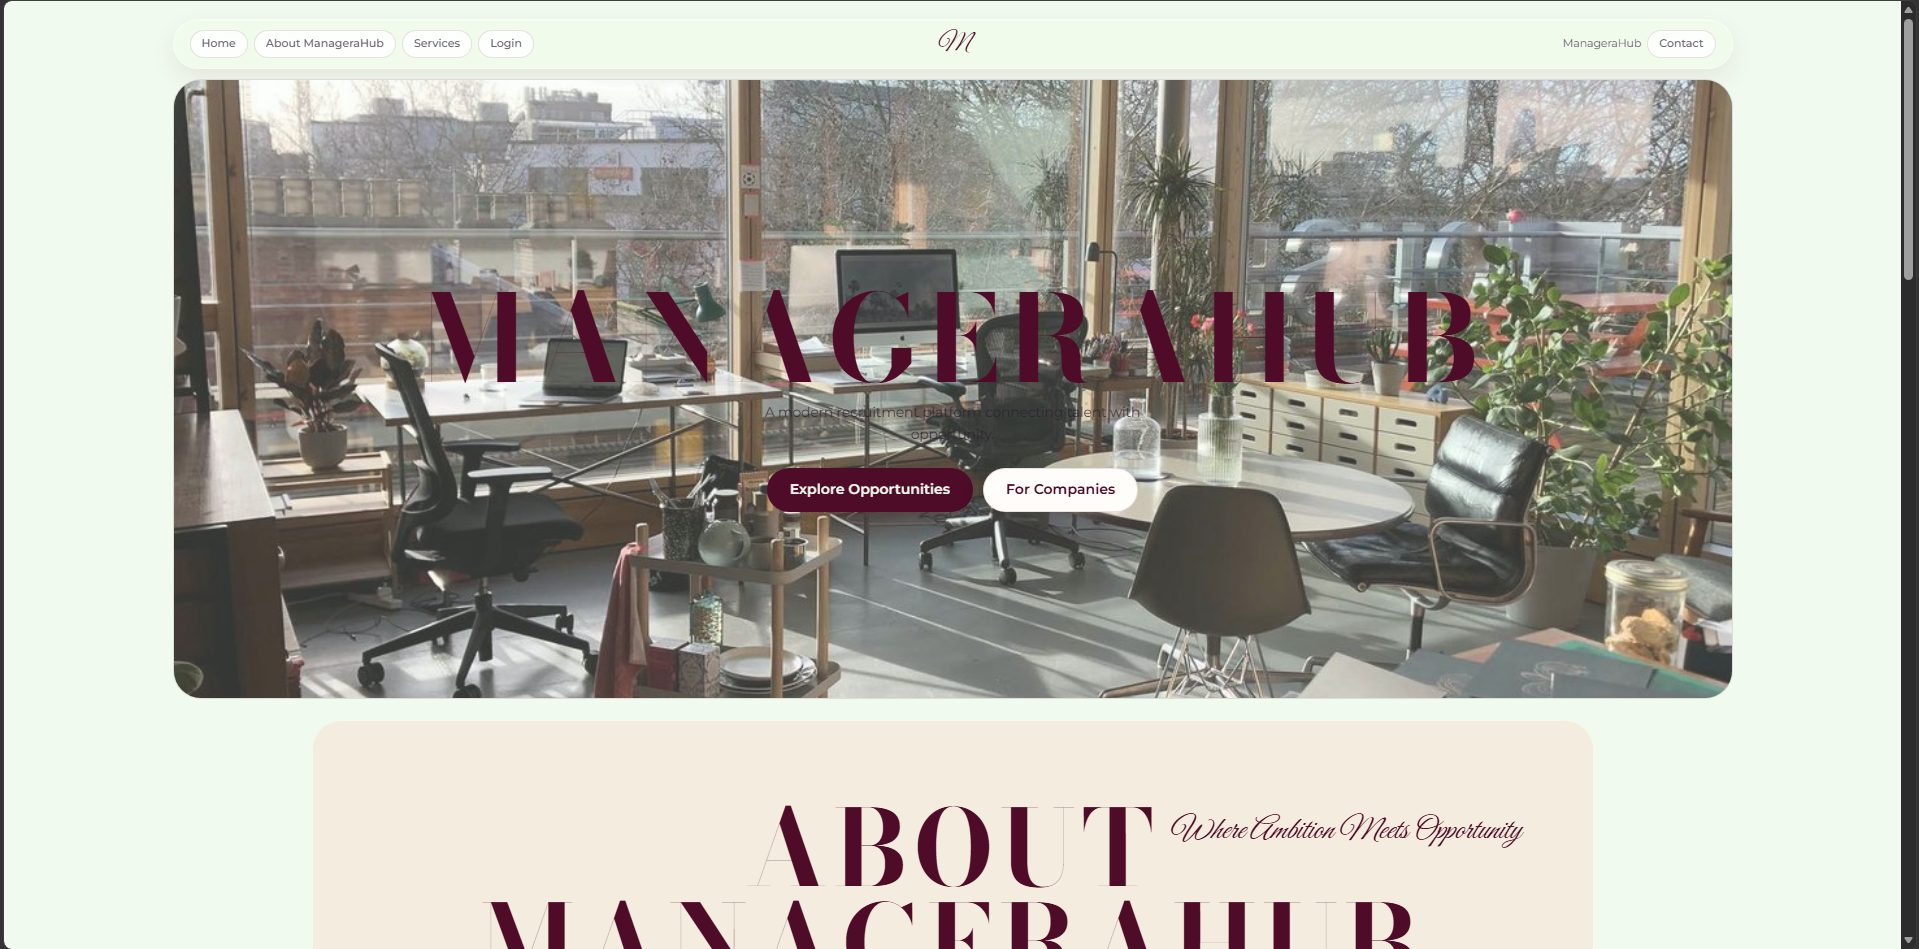
\includegraphics[width=\textwidth]{diagrams/landing.png}
    \caption{Page d'accueil de ManageraHub - Vue Desktop}
    \label{fig:landing_desktop}
\end{figure}

\begin{figure}[H]
    \centering
    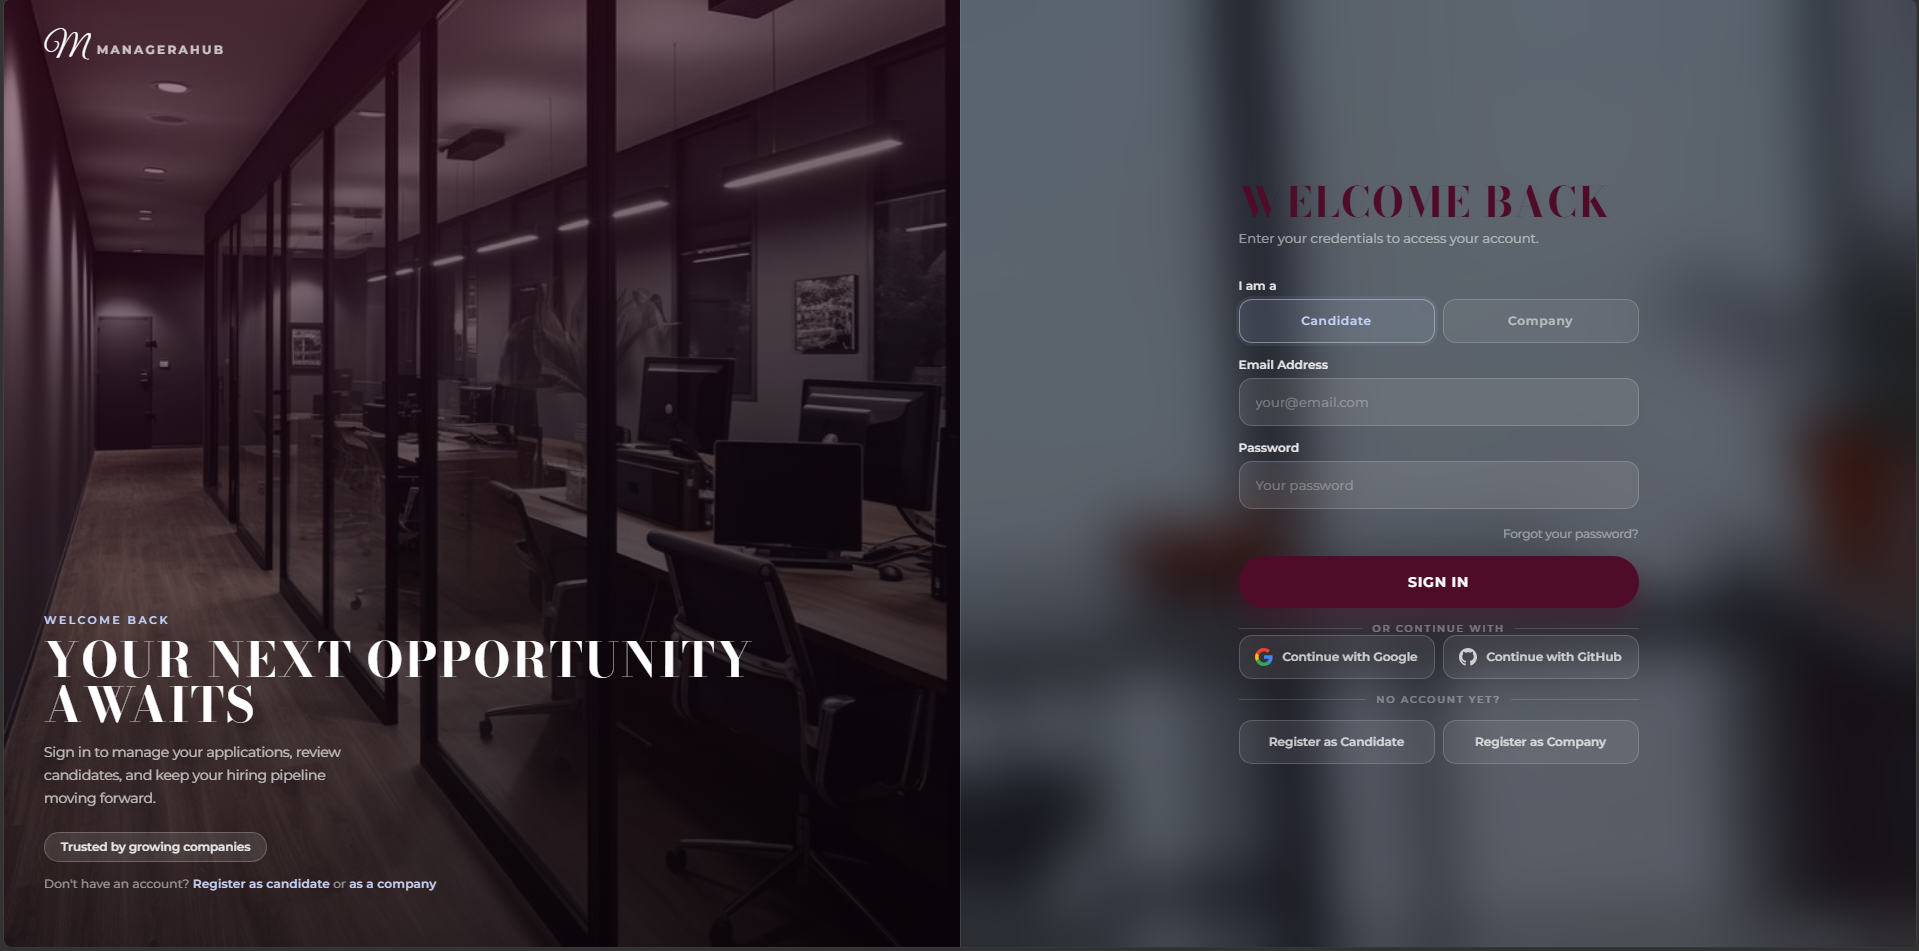
\includegraphics[width=\textwidth]{diagrams/signin.png}
    \caption{Interface de Connexion et d'Inscription de ManageraHub}
    \label{fig:signin_page}
\end{figure}

\subsection{2. Espace Candidat et Tableaux de Bord}
L'espace Candidat affiche un tableau de bord complet avec le pourcentage de complétion de son profil, sa liste de candidatures actives et leurs statuts.

De plus, nous y avons intégré un module de \textbf{suivi en temps réel des candidatures (Application Tracker)}. Ce widget de type carrousel permet au candidat de visualiser graphiquement l'évolution de ses demandes via une frise chronologique interactive (étapes : \textit{Candidature envoyée, Examen en cours, Entretien planifié, Décision finale}). Les données sont synchronisées automatiquement en tâche de fond (polling asynchrone) sans nécessiter de rafraîchir manuellement la page. Si un changement d'état est détecté, un indicateur visuel de scan radar s'active temporairement et applique un effet de surbrillance lumineuse sur la frise.

Le candidat accède également au \textbf{fil d'actualité social professionnel (Social Feed)}, optimisé pour l'interactivité grâce au défilement infini (Infinite Scroll), à l'apparition progressive par squelettes de chargement (skeletons loaders), et à l'autocomplétion dynamique lors de la recherche de membres ou de tags.

\begin{figure}[H]
    \centering
    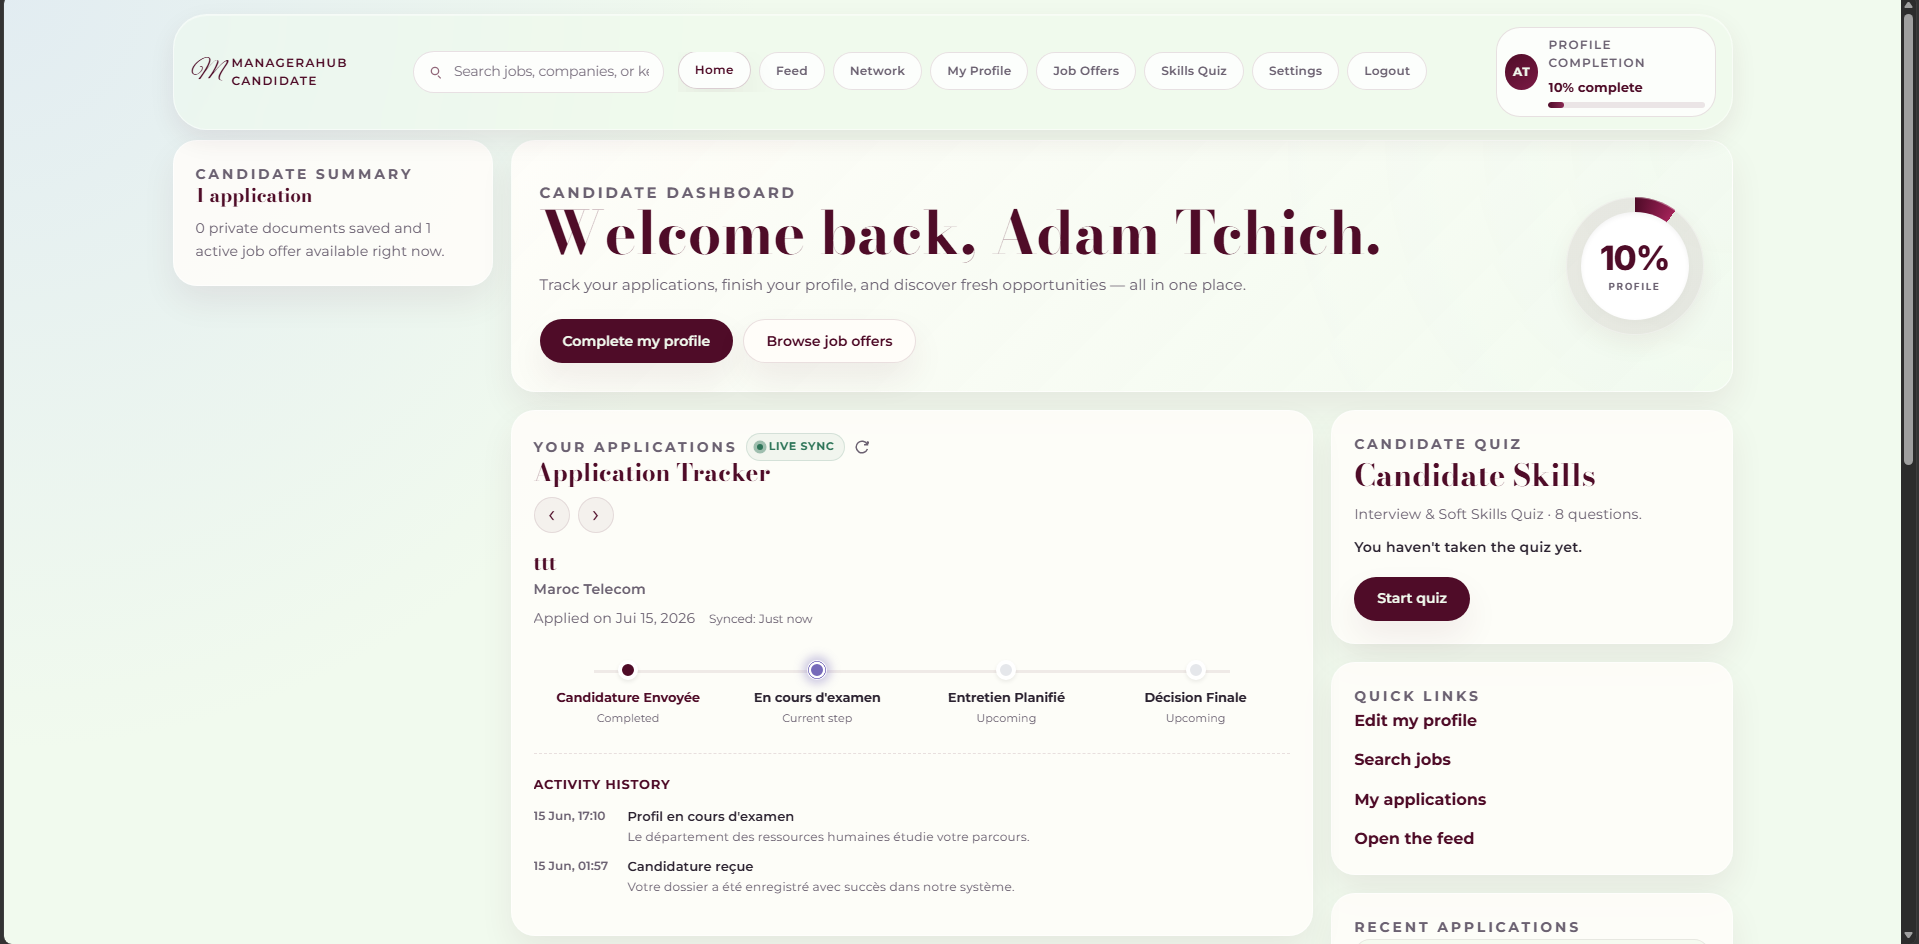
\includegraphics[width=\textwidth]{diagrams/candidate_dashboard.png}
    \caption{Tableau de bord de l'Espace Candidat avec barre de progression de profil}
    \label{fig:cand_dashboard}
\end{figure}

\begin{figure}[H]
    \centering
    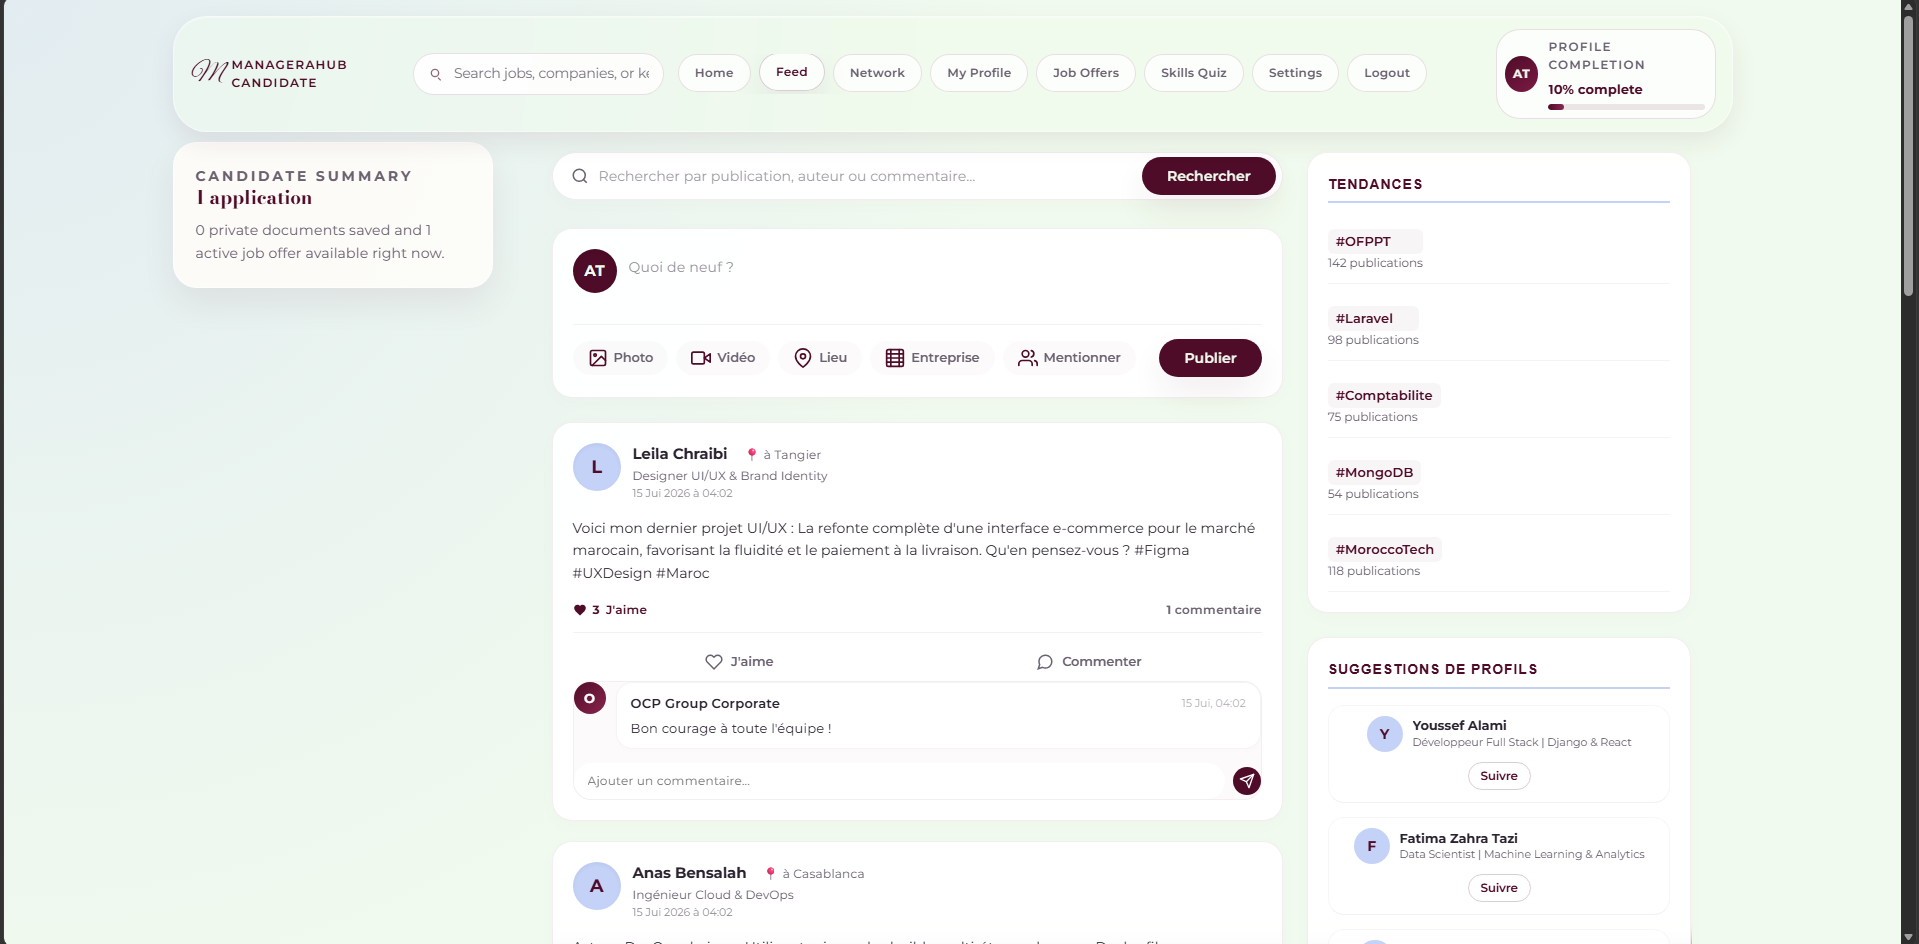
\includegraphics[width=\textwidth]{diagrams/feed.png}
    \caption{Fil d'actualités social de la plateforme avec likes et commentaires}
    \label{fig:social_feed}
\end{figure}

\subsection{3. Espace Entreprise et Gestion des Offres}
L'entreprise accède à un espace restreint permettant de gérer ses offres d'emploi actives et d'analyser les dossiers de candidature reçus.

\begin{figure}[H]
    \centering
    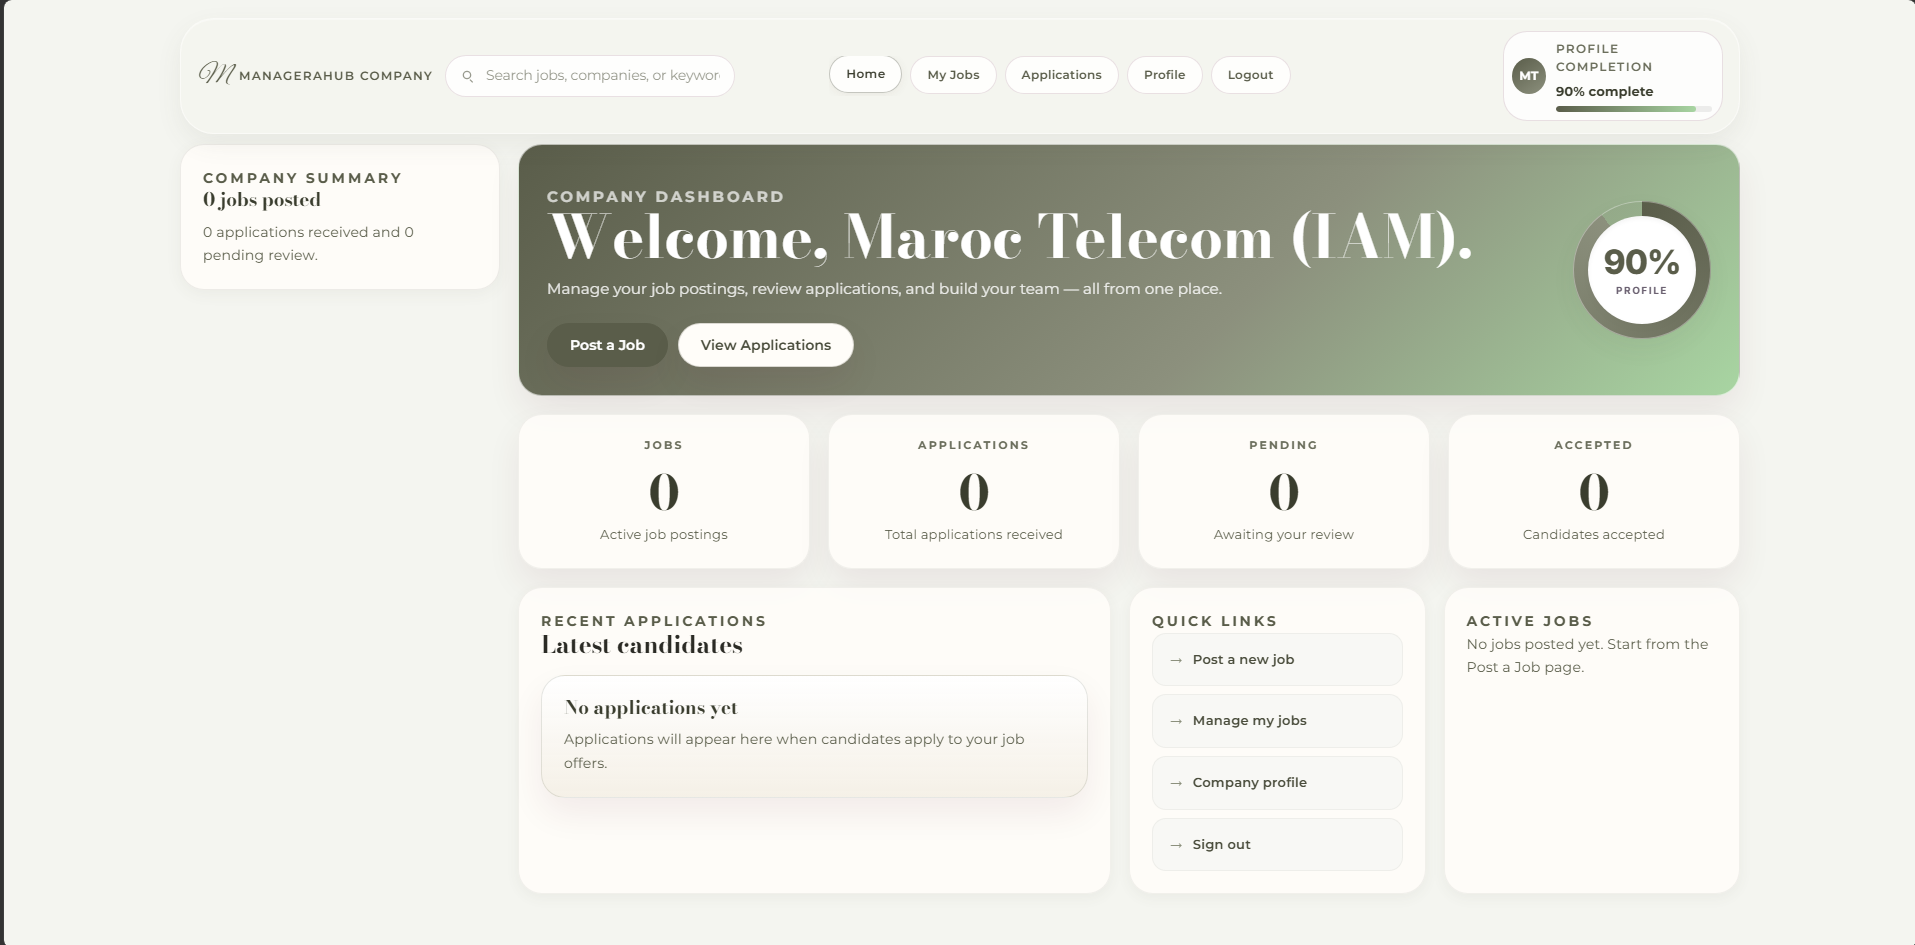
\includegraphics[width=\textwidth]{diagrams/company_dashboard.png}
    \caption{Tableau de bord de pilotage d'une Entreprise approuvée}
    \label{fig:comp_dashboard}
\end{figure}

\begin{figure}[H]
    \centering
    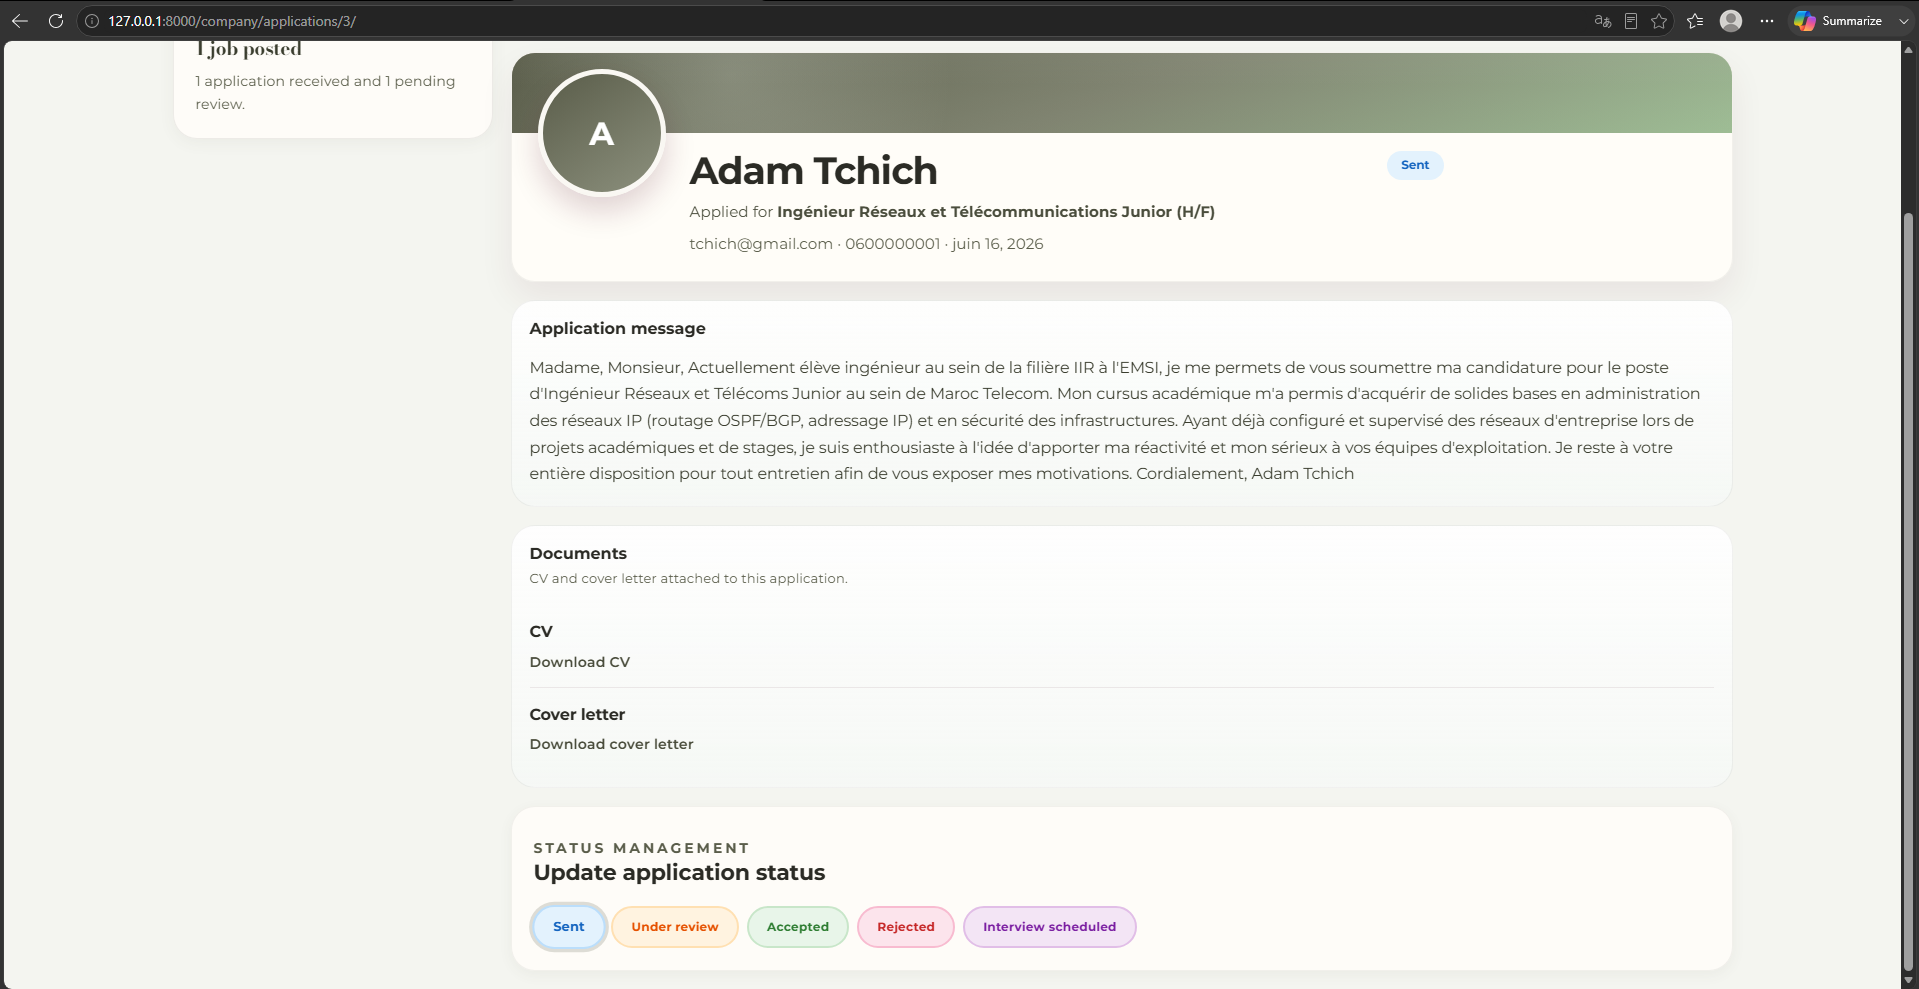
\includegraphics[width=\textwidth]{diagrams/company_application_detail.png}
    \caption{Écran d'évaluation des candidatures et de changement de statut}
    \label{fig:comp_app_detail}
\end{figure}

\subsection{4. Espace d'Administration et Modération}
Le panneau de contrôle de l'administrateur permet de vérifier les documents de légitimité de l'entreprise (ICE et RC) avant d'activer le compte.

\begin{figure}[H]
    \centering
    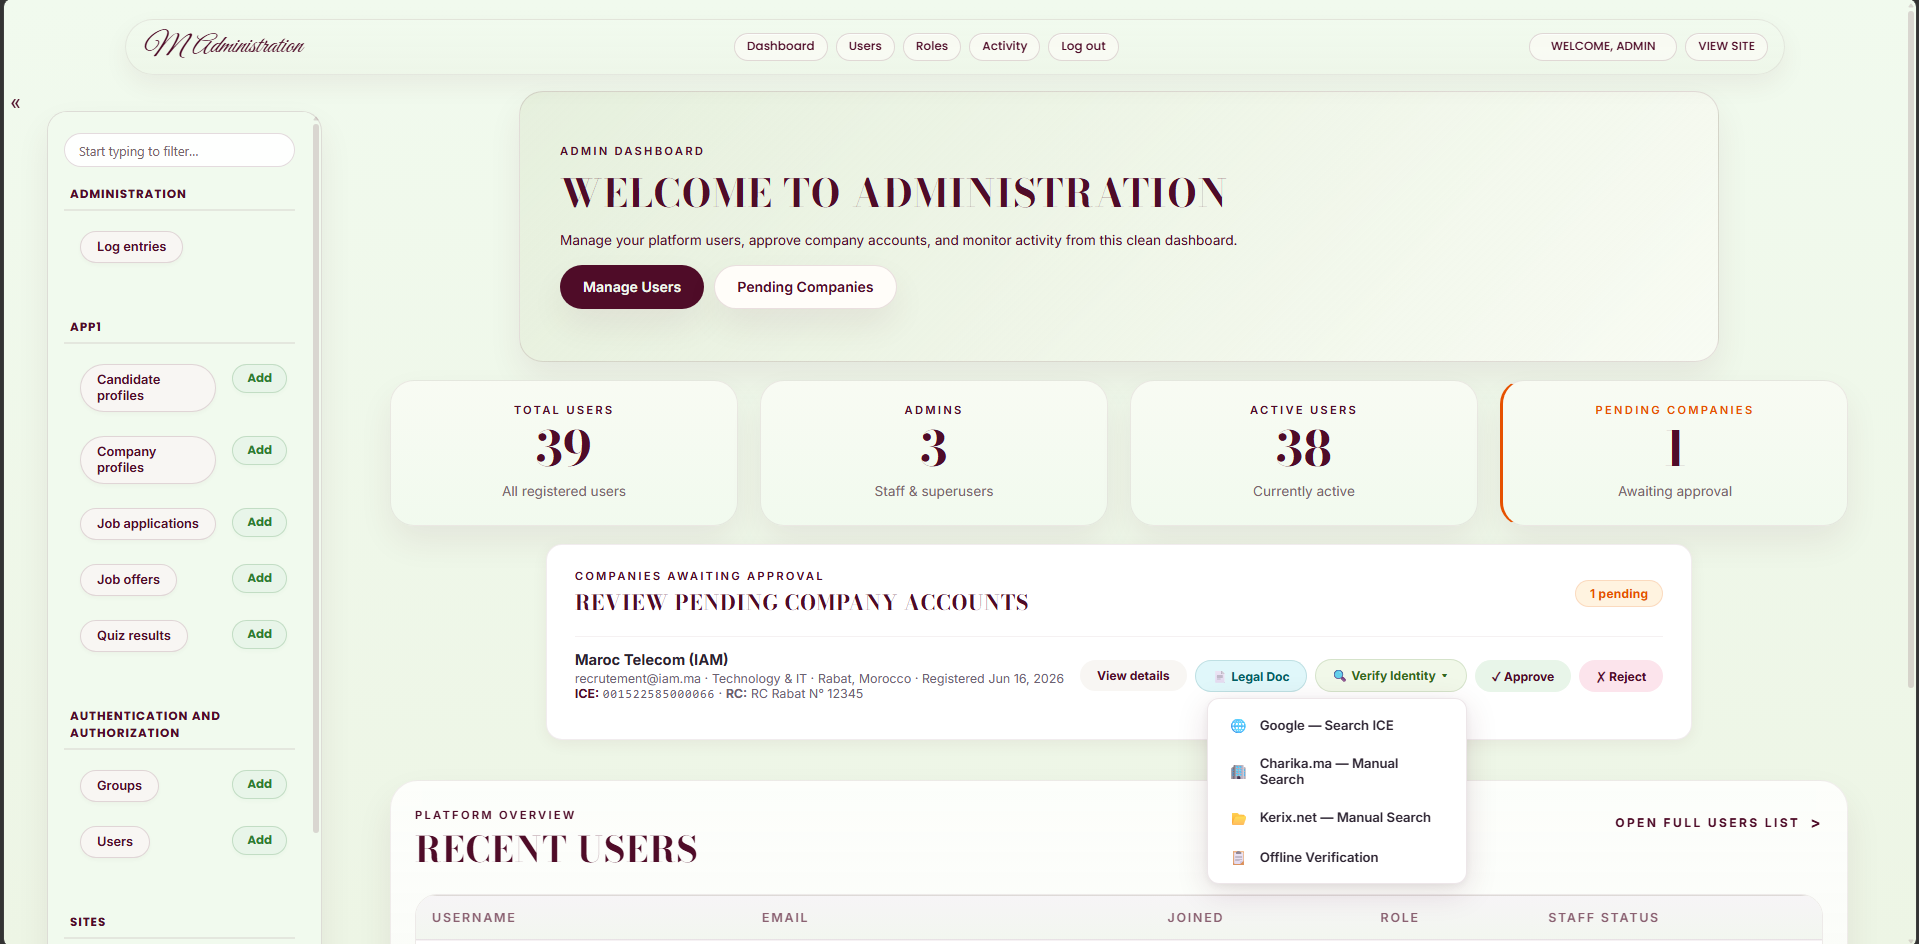
\includegraphics[width=\textwidth]{diagrams/admin_dashboard.png}
    \caption{Panneau d'administration - Validation des comptes recruteurs}
    \label{fig:admin_validation}
\end{figure}

\subsection{5. Version Mobile (Responsive Design)}
Tous les éléments graphiques se réorganisent sur les écrans mobiles et tablettes pour garantir un centrage et une lisibilité optimale.

\begin{figure}[H]
    \centering
    \includegraphics[width=\textwidth]{diagrams/mobile_responsive.png}
    \caption{Rendu de l'application ManageraHub sur écran de Smartphone}
    \label{fig:responsive_mobile}
\end{figure}

\section{Sécurité applicative mise en œuvre}
Le framework Django intègre nativement des protections contre les vulnérabilités courantes du web. Nous avons configuré et vérifié ces mécanismes :
\begin{itemize}
    \item \textbf{Protection CSRF (Cross-Site Request Forgery) :} Tous les formulaires POST génèrent un jeton unique vérifié côté serveur.
    \item \textbf{Protection XSS (Cross-Site Scripting) :} Le moteur de rendu de gabarit Django échappe automatiquement les balises HTML et JavaScript non autorisées.
    \item \textbf{Hashage des mots de passe :} Utilisation du hashage itératif PBKDF2 avec sel dynamique pour le stockage des identifiants utilisateurs.
\end{itemize}

\section{Difficultés rencontrées et solutions apportées}
Durant la phase finale d'intégration de la charte graphique et de mise en œuvre du responsive design, plusieurs défis techniques ont dû être surmontés :
\begin{enumerate}
    \item \textbf{Alignement et centrage des formulaires et des tableaux de bord :} Sur les terminaux mobiles et tablettes, certains formulaires d'authentification et de profilage apparaissaient décentrés ou présentaient des problèmes de débordement horizontal. Nous avons résolu cela en restructurant nos feuilles de style (\texttt{static/css/main.css}) pour utiliser un système de grille CSS (CSS Grid) et de boîte flexible (Flexbox) avec des marges auto-calculées, garantissant un centrage géométrique parfait de tous les boutons et entrées sur mobile.
    \item \textbf{Gestion des documents légaux :} L'ICE de l'entreprise doit obligatoirement faire 15 chiffres. Nous avons développé des validateurs personnalisés côté modèle Django (en utilisant des expressions régulières \texttt{RegexValidator}) pour bloquer l'enregistrement de valeurs invalides directement lors de la soumission du formulaire d'inscription entreprise.
    \item \textbf{Fichiers médias :} Les CV, photos de profil et lettres de motivation contiennent des informations personnelles. Pour éviter qu'ils ne soient mélangés, nous avons implémenté des fonctions de génération de chemins de stockage dynamiques et compartimentés (comme les fonctions de stockage de profil ou de candidature) qui organisent automatiquement les téléversements dans des répertoires sécurisés par identifiants d'utilisateurs et d'offres.
    \item \textbf{Mise à jour d'état en temps réel (Tracker) :} Interroger intensivement le serveur pour actualiser la timeline de candidature peut surcharger la base de données. Nous avons résolu ce problème en développant un point d'API Django dédié et optimisé qui renvoie uniquement les données JSON nécessaires, couplé à une scrutation (polling) asynchrone côté client. De plus, l'overlay de scan radar ne s'active visuellement que lorsqu'une réelle transition d'état est détectée en base de données, alliant fluidité et économie de requêtes.
    \item \textbf{Expérience fluide du fil d'actualité (Social Feed) :} Le chargement d'un grand nombre de publications avec images et vidéos ralentissait l'affichage global sur mobile. Nous avons implémenté une pagination dynamique par défilement infini (Infinite Scroll) en JavaScript. Pour combler le temps de chargement asynchrone, nous avons conçu des squelettes de chargement (skeletons loaders) animés en CSS, masquant le délai réseau et rendant l'interface fluide.
\end{enumerate}

\section{Conclusion}
La phase de réalisation s'est achevée par des phases de tests fonctionnels unitaires validant l'ensemble de la logique métier. La plateforme ManageraHub se révèle stable, sécurisée et conforme aux spécifications du cahier des charges académique.
\newpage
